\documentclass[12pt, a4paper, twoside]{article}
\usepackage[utf8]{inputenc}
\usepackage{graphicx}
\graphicspath{ {images/} }
\PassOptionsToPackage{hyphens}{url}
\usepackage{hyperref}
\usepackage{rotating}
\usepackage{pdflscape}
\usepackage{amsmath}
\usepackage{cancel}



\title{CalculiX Benchmark Study:\\Two-Dimensional Blisk}
\author{Süleyman Muti}
\date{May 19, 2020}

\begin{document}


\maketitle


\begin{abstract}	
The analytical and finite element analysis results of a two-dimensional rotating blisk problem are compared. The free and open-source finite element analysis software CalculiX is used. The blisk is modelled using axisymmetric elements for the disk portion and plane strain elements for the blade portion.
\end{abstract}


\section{Rotating Blisk Problem}

Consider the following two-dimensional rotating blisk (disk with integral blades) problem shown in Figure ~\ref{fig:parametric_blisk} based on Reference \cite{rotors_book}. 

\begin{figure}[h]
	\centering
	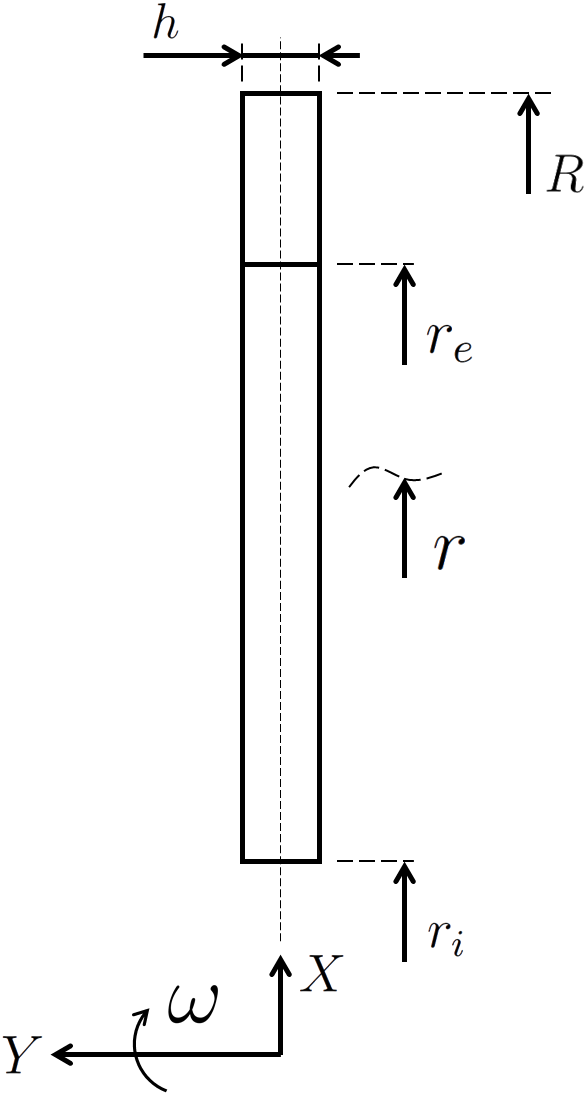
\includegraphics[scale=0.2]{parametric_blisk}
	\caption{Parametric rotating blisk.}
	\label{fig:parametric_blisk}
\end{figure}

There are $N$ number of blades in $360^\circ$. Blades are rectangular prisms and span from $r_e$ to $R$, i.e., the blade height is  $R-r_e$. The blisk is made of a linear elastic metal with an elasticity modulus of $E$, Poisson's ratio of $\nu$, and density of $\gamma$. A blade has a width of w.

Following ratio between the total volume of the blades and the volume of the corresponding solid ring between radii $r_e$ and $R$ apply.

\begin{equation}
	\label{equation:volume_ratio}
	k{=}{\frac {{V}_{blades}} {{V}_{ring}}}, \quad 0{<}k{<}1.
\end{equation}

Using the following given parameters, calculate the radial stresses, hoop stresses, and radial displacements along the blisk symmetry axis between the bore and hub radii.\\

Geometry:

$r_i$ $=$ $100$ $mm$,

$r_e$ $=$ $400$ $mm$,

$R$ $=$ $660$ $mm$,

$h$ $=$ $10$ $mm$,

$N$ $=$ $24$,

$k$ $=$ $0.5$.\\


Material properties:

$E$ $=$ $2.1 \times 10^{5}$ $MPa$,

$\nu$ $=$ $0.3$,

$\gamma$ $=$ $7.8 \times 10^{-9}$  $tonne/mm^{3}$.\\


Loading:

$\omega$ $=$ $1800$ $rpm$.\\

The problem geometry with given parameters is illustrated in Figure ~\ref{fig:blisk_with_given_parameters}. 

\begin{figure}[h]
	\centering
	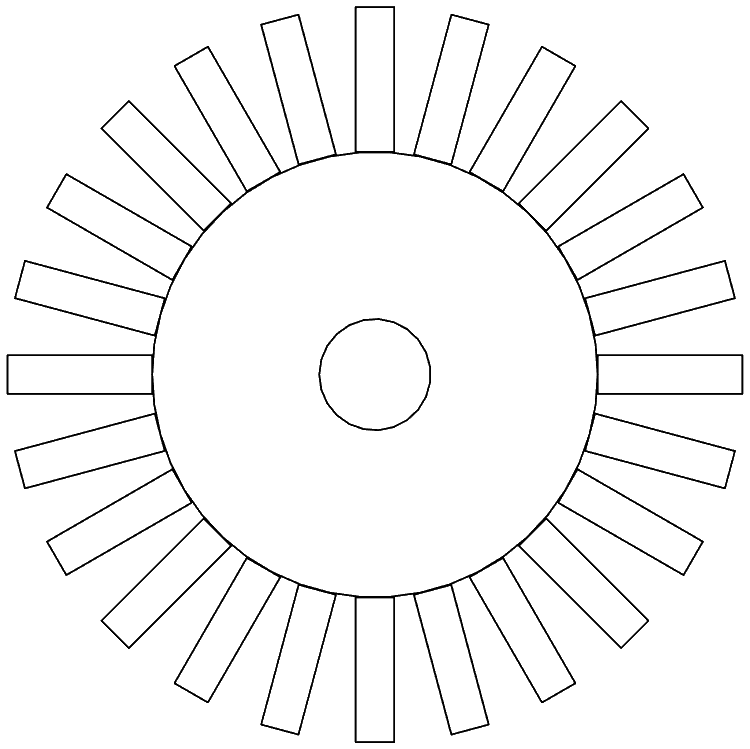
\includegraphics[scale=0.2]{blisk_with_given_parameters}
	\caption{Rotating blisk with given parametric values.}
	\label{fig:blisk_with_given_parameters}
\end{figure}


\section{\sloppy Solution: The Theory of Elasticity}

The rotating blisk problem can be considered as the superposition of two elastic problems.

\begin{itemize}
	\item Non-rotating annular disk with radial stress applied at the outer radius,
	\item Rotating annular disk of same size.
\end{itemize}

The rotating blisk cannot carry hoop stress between the hub radius $r_e$ and tip radius $R$. The centrifugal force due to the rotating mass of the blades is reflected as a boundary condition to the non-rotating annular disk problem.\\

\noindent
\textbf{Solution to non-rotating annular disk loaded at the outer radius:}

The solution is given by the following equations \cite{rotors_book}.

\begin{equation}
	\label{equation:nr_sigma_r}
	{{\sigma }_{r}}={{\sigma }_{re}}{\frac {1} {1-{{\beta }^{2}}}}\left ( {1-{\frac {{\beta }^{2}} {{\rho }^{2}}}} \right )
\end{equation}

\begin{equation}
	\label{equation:nr_sigma_t}
	{{\sigma }_{t}}={{\sigma }_{re}}{\frac {1} {1-{{\beta }^{2}}}}\left ( {1+{\frac {{\beta }^{2}} {{\rho }^{2}}}} \right )
\end{equation}

\begin{equation}
	\label{equation:nr_u_r}
	{{u}_{r}}={{\sigma }_{re}}{\frac {{r}_{e}} {E}}{\frac {\rho } {1-{{\beta }^{2}}}}\left [ {\left ( {1-{\nu }} \right )+\left ( {1+{\nu }} \right ){\frac {{\beta }^{2}} {{\rho }^{2}}}} \right ]
\end{equation}

\noindent
\textbf{Solution to rotating annular disk problem:}


The solution is given by the following equations \cite{rotors_book}.

\begin{equation}
	\label{equation:r_sigma_r}
	{{\sigma }_{r}={\frac {(3+{\nu })} {8}{{\sigma }_{0}}}\left ( {1+{{\beta }^{2}}-{\frac {{\beta }^{2}} {{\rho }^{2}}-{\rho }^{2}}} \right )}
\end{equation}

\begin{equation}
	\label{equation:equation:r_sigma_t}
	{{\sigma }_{t}={\frac {(3+{\nu })} {8}{{\sigma }_{0}}}\left ( {1+{{\beta }^{2}}+{\frac {{\beta }^{2}} {{\rho }^{2}}-{\frac {\left ( {1+3{\nu }} \right )} {\left ( {3+{\nu }} \right )}}{\rho }^{2}}} \right )}
\end{equation}

\begin{equation}
	\label{equation:r_u_r}
	{{u}_{r}}={\frac {{r}_{e}} {E}}{{\rho }\frac {\left ( {3+{\nu }} \right )} {8}}{{\sigma }_{0}}\left [ {\left ( {1+{{\beta }^{2}}} \right )\left ( {1-{\nu }} \right )+\left ( {1+{\nu }} \right ){\frac {{\beta }^{2}} {{\rho }^{2}}}-{{\rho }^{2}}\left ( {{\frac {1-{{\nu }^{2}}} {3+{\nu }}}} \right )} \right ]
\end{equation}

where

$\rho$ $=$ $r/r_e$,

$\beta$ $=$ $r_i/r_e$,

$\sigma_{re}$ $=$ $\sigma_r|_{r_e}$, 

$\sigma_0$ $=$ $\gamma{\omega}^{2}{r_e}^{2}$.\\

\noindent
\textbf{The radial stress at hub radius $r_e$:}\\

The radial stress at hub radius $r_e$ is given by Equation  ~\ref{equation:sigma_r_at_re}.

\begin{equation}
	\label{equation:sigma_r_at_re}
	{\sigma}_{re}=\frac{F_c}{A_{r_e}}
\end{equation}

\noindent
where $F_c$ is the centrifugal force due to the rotating mass of the blades, and ${A_{r_e}}$ is the area of the cylindrical surface at the hub radius $r_e$.\\


The centrifugal force due to the rotating mass of the blades is given by Equation  ~\ref{equation:cent_force_re}.

\begin{equation}
	\label{equation:cent_force_re}
	F_c=\frac{ k \gamma \pi h (R^2-{r_e}^2) {\omega}^2 (R + r_e) }{2}
\end{equation}


The area of the cylindrical surface at the hub radius $r_e$ is given by Equation  ~\ref{equation:area_at_re}.

\begin{equation}
	\label{equation:area_at_re}
	{A_{r_e}=2 \pi h r_e}
\end{equation}

The radial stress at hub radius $r_e$ is obtained by substituting Eqs. ~\ref{equation:cent_force_re} and ~\ref{equation:area_at_re} into Eq. ~\ref{equation:sigma_r_at_re}.

\begin{equation}
	\label{equation:sigma_r_at_re_ii}
	\begin{aligned}
		{\sigma}_{re} & =\frac{ k \gamma \pi h {\omega}^2 (R^2-{r_e}^2) (R + r_e) }{4 \pi h r_e}\\
		& =\frac{ k \gamma {\omega}^2 (R^2-{r_e}^2) (R + r_e) }{4 r_e}
	\end{aligned}
\end{equation}

The radial stress value at hub radius $r_e$ is obtained by substituting the given parameter values into Equation ~\ref{equation:sigma_r_at_re_ii}.

\begin{equation}
	\label{equation:sigma_r_val_at_re}
	{\sigma}_{re} = 25.3\:MPa
\end{equation}

\noindent
\textbf{The reference stress $\sigma_0$}:\\

\begin{equation}
	\label{equation:sigma_0_val_at_re}
	\begin{aligned}
		{\sigma}_{0} &= \gamma{\omega}^{2}{r_e}^{2}\\
		&= 44.34\:MPa
	\end{aligned}
\end{equation}

A MATLAB code is written to calculate and plot the radial stresses, hoop stresses, and radial displacements along the blisk symmetry axis from the bore radius $r_i$ to te hub radius $r_e$. The radial and hoop stresses are shown in Figure ~\ref{fig:analytical_solution_stress}, and the radial displacements are shown in Figure ~\ref{fig:analytical_solution_disp}.

\begin{figure}[h]
	\centering
	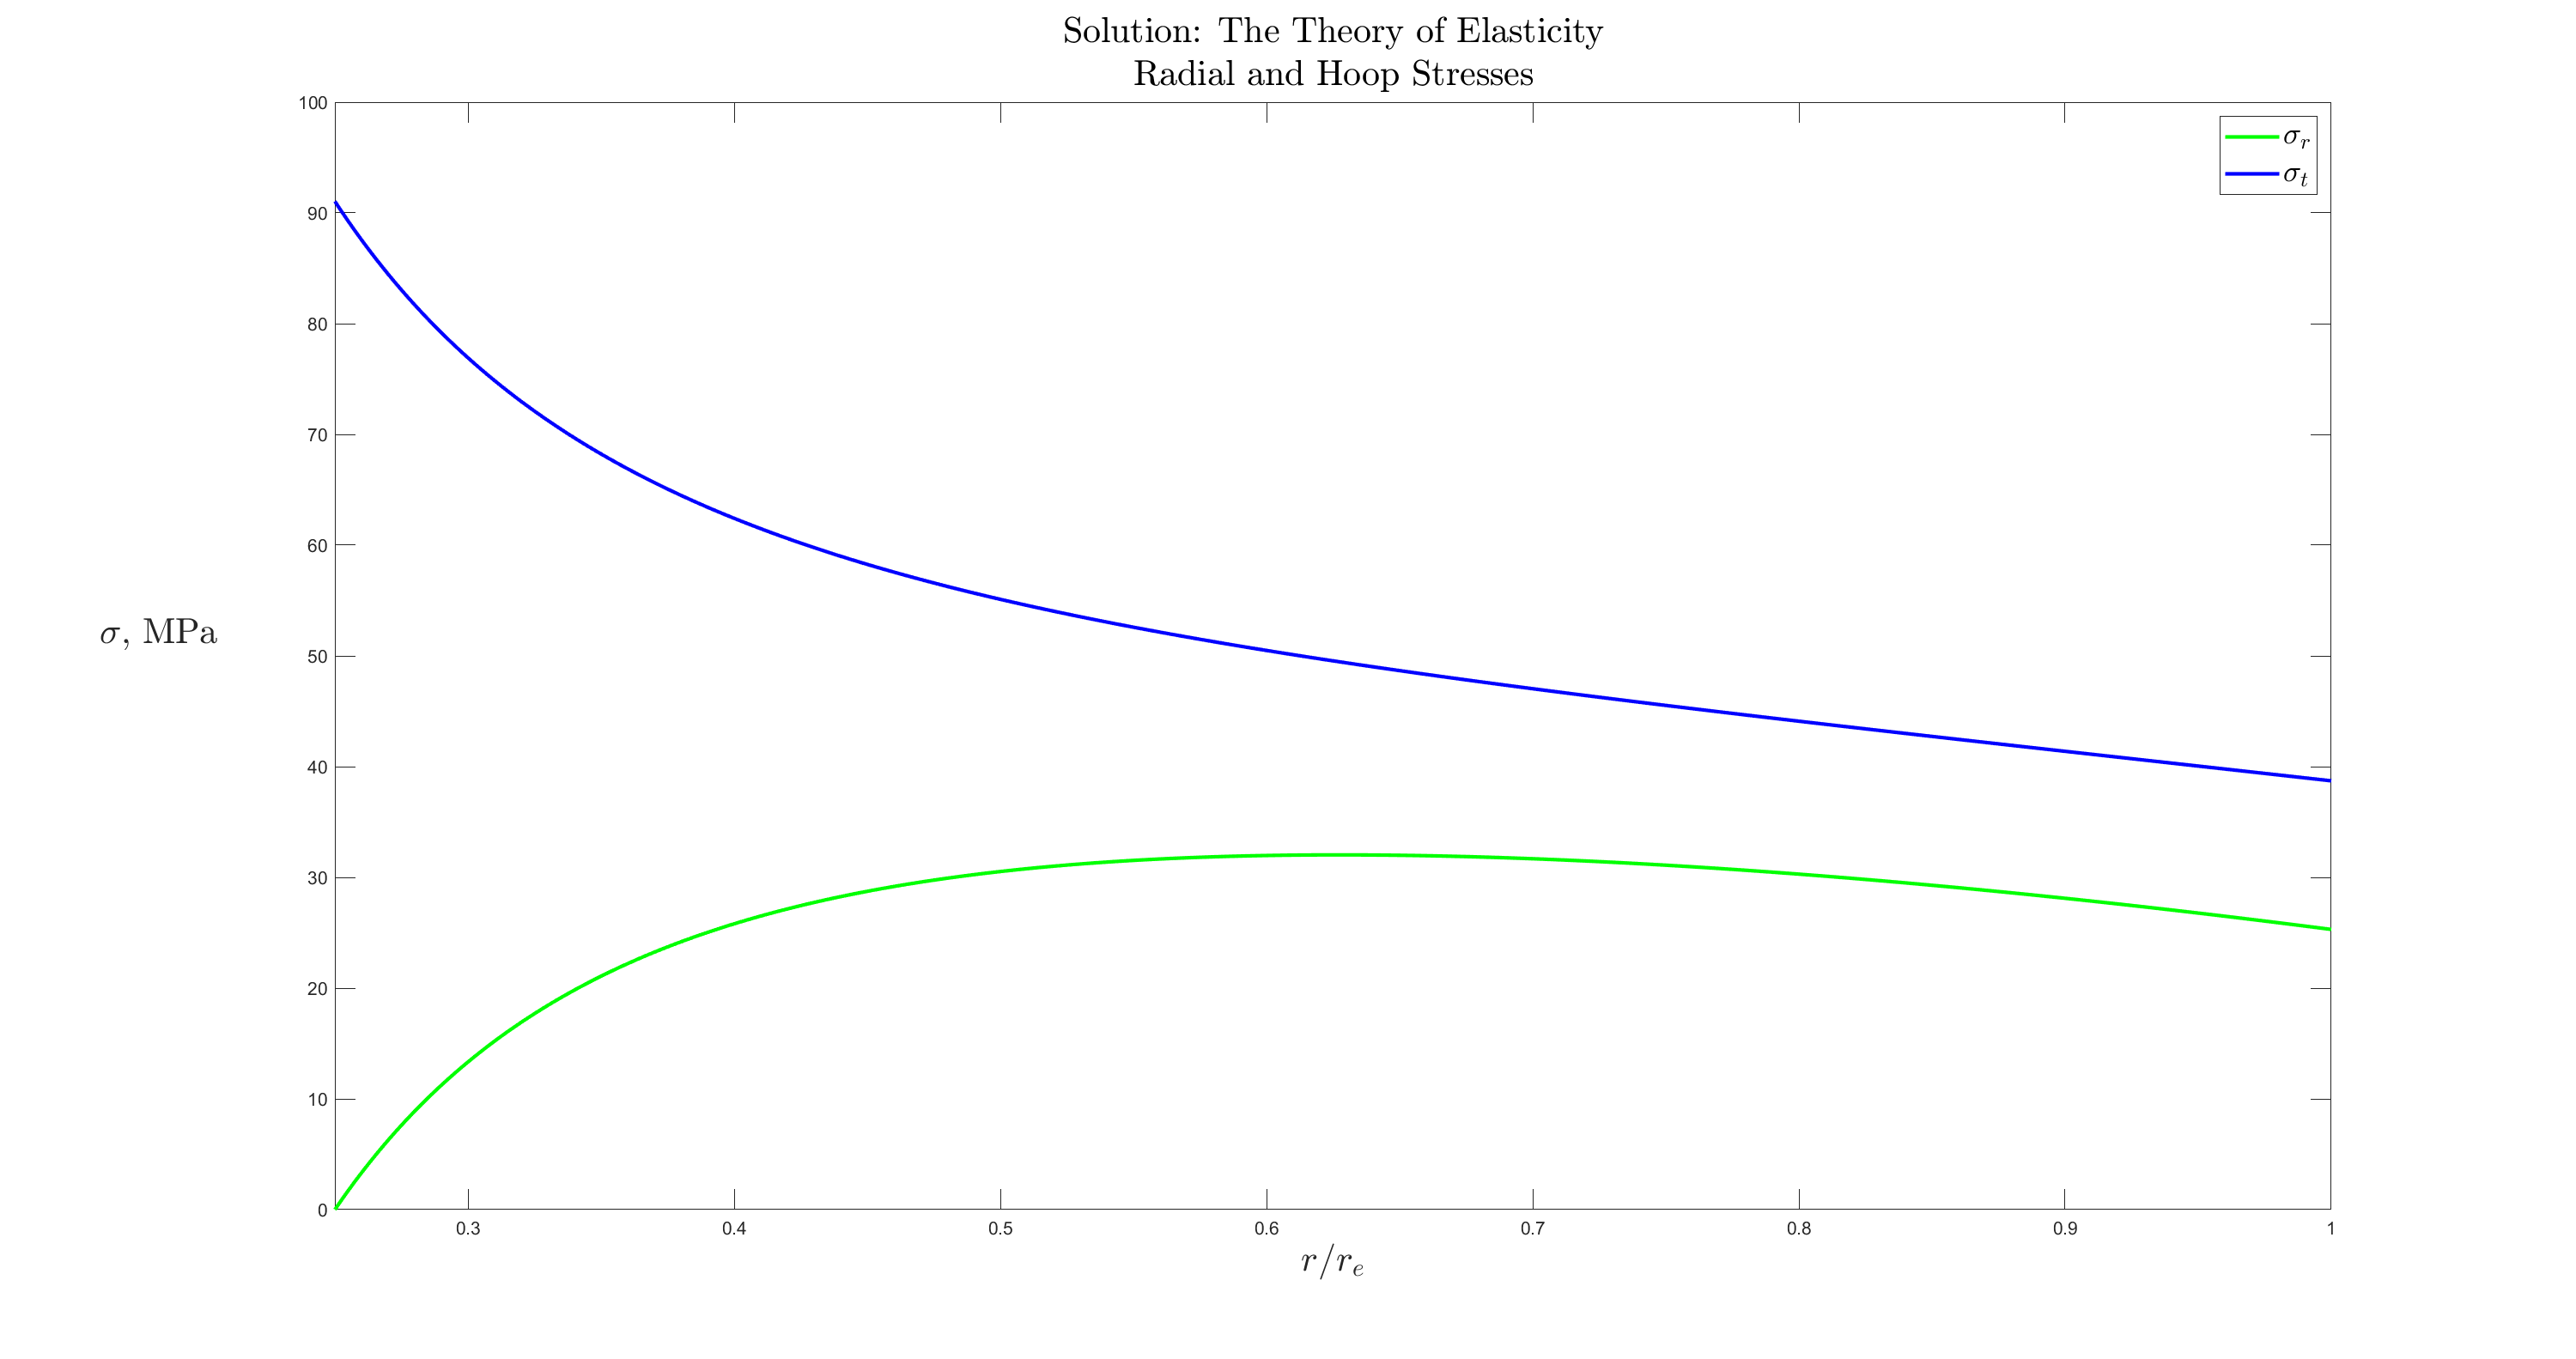
\includegraphics[scale=0.25]{analytical_solution_stress}
	\caption{Theory of Elasticity solution for radial and hoop stresses.}
	\label{fig:analytical_solution_stress}
\end{figure}

\begin{figure}[h]
	\centering
	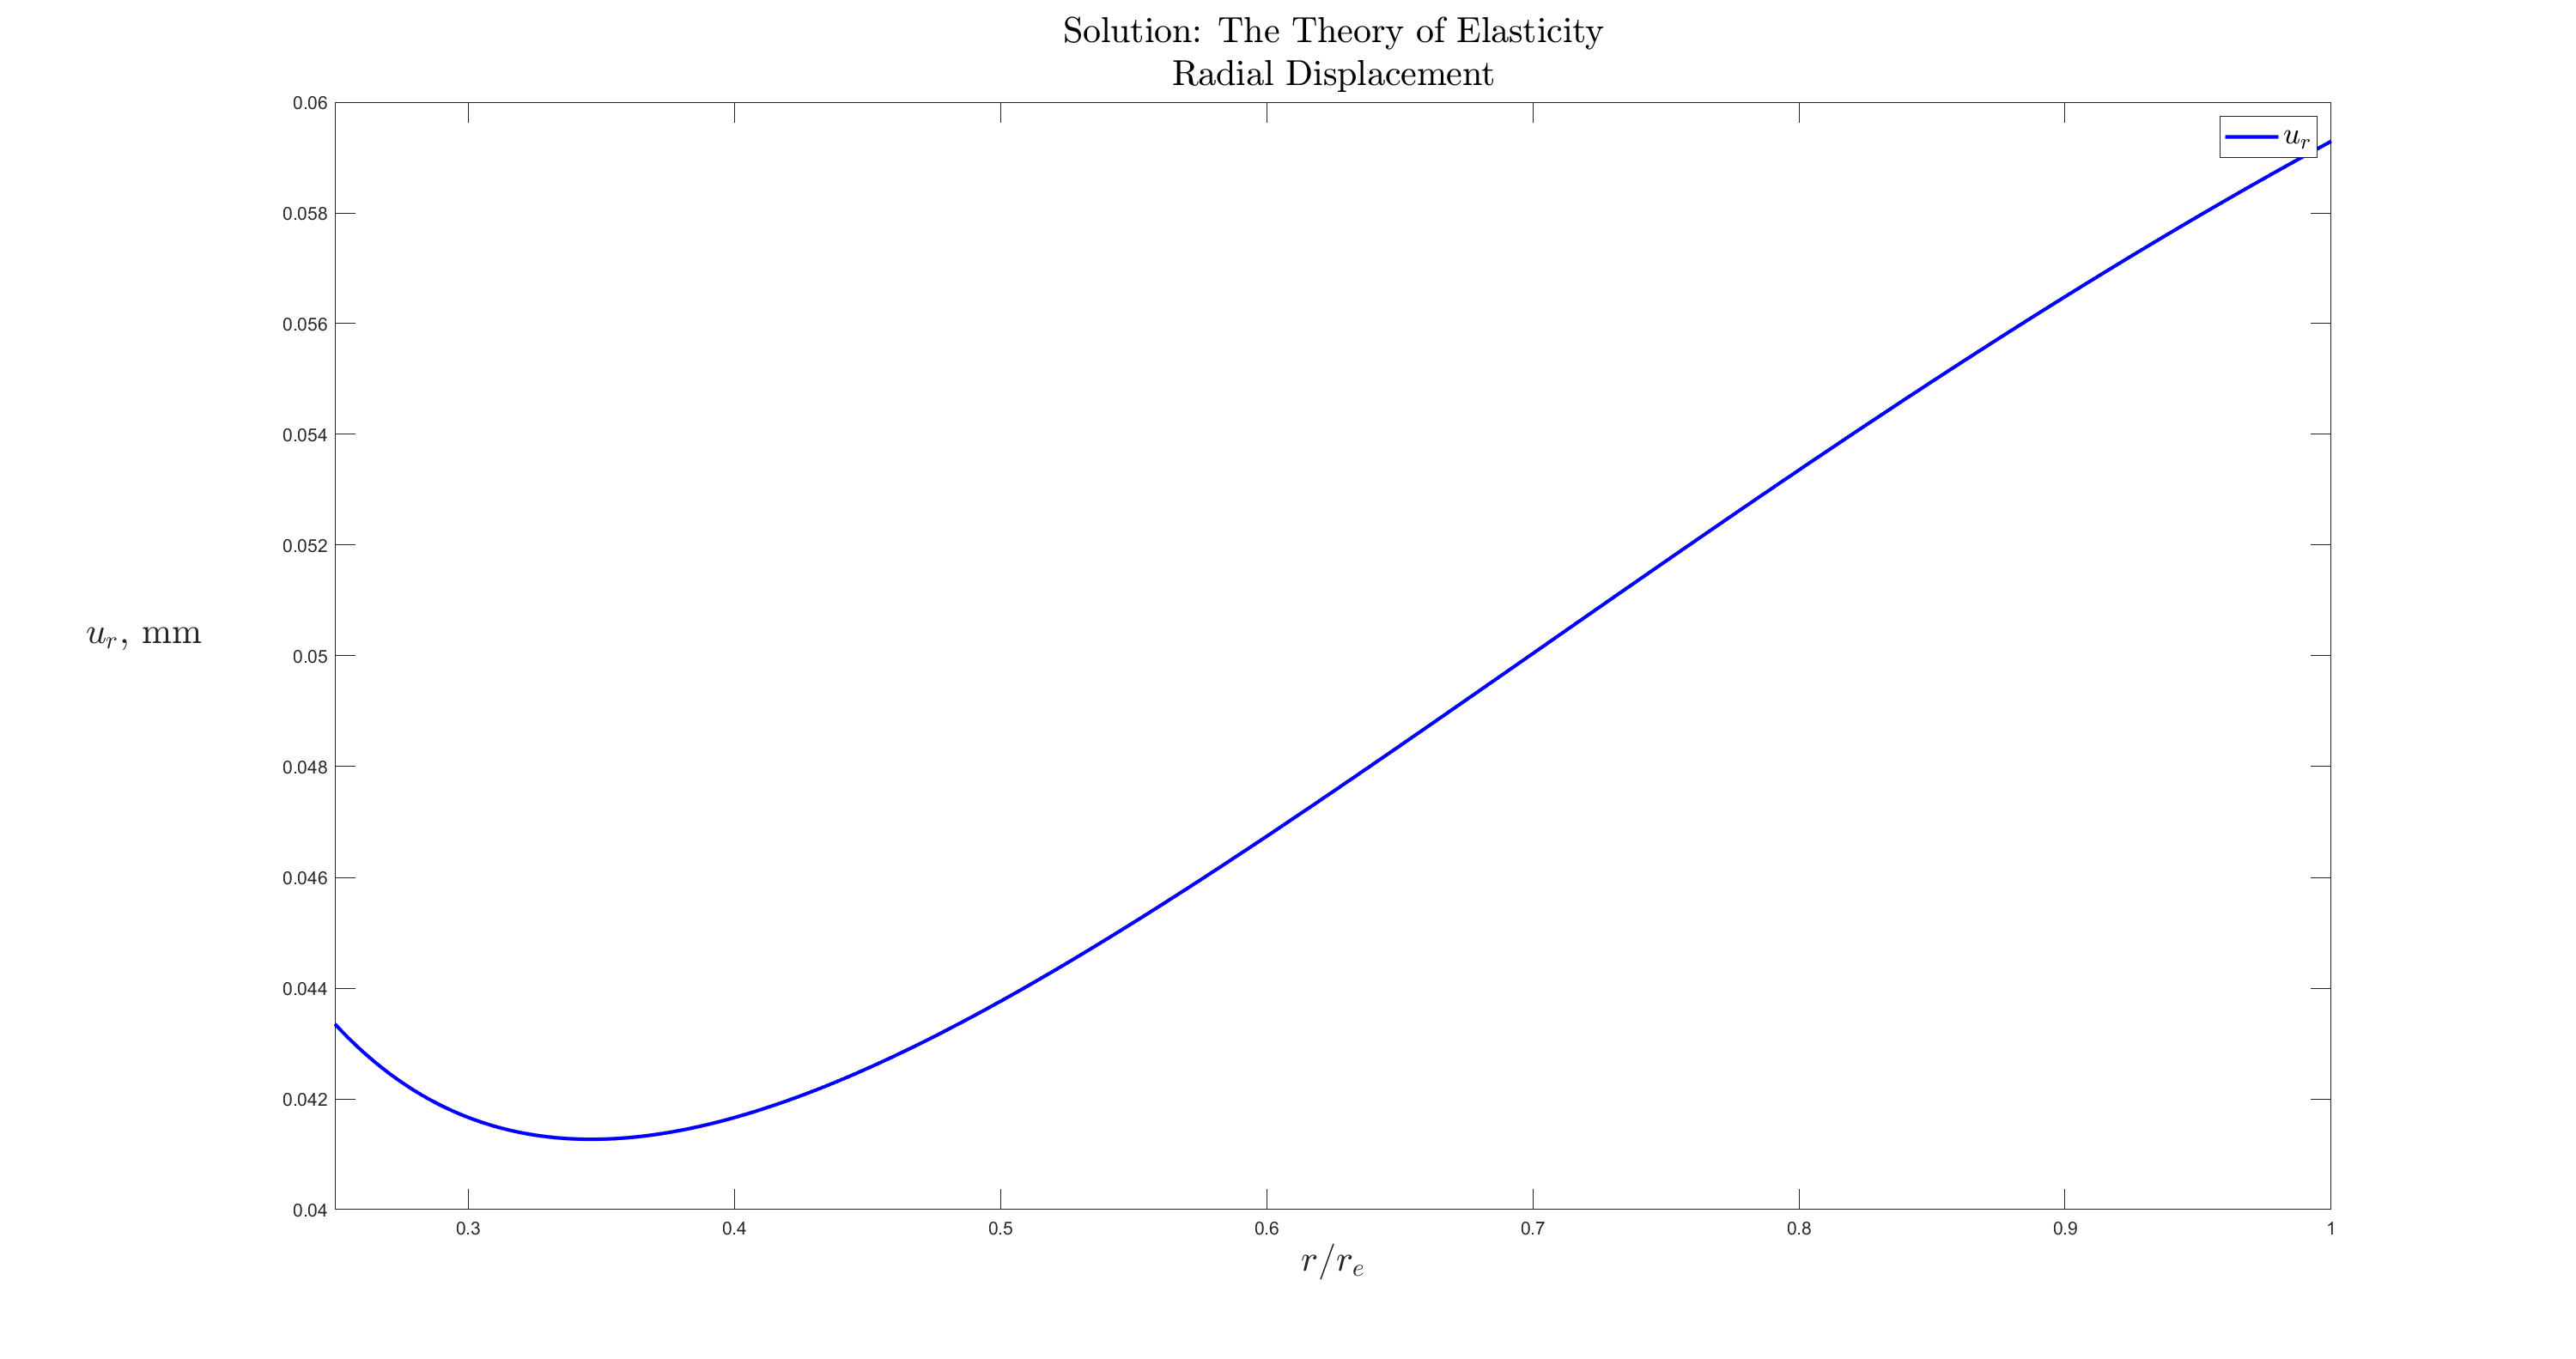
\includegraphics[scale=0.25]{analytical_solution_disp}
	\caption{Theory of Elasticity solution for radial displacements.}
	\label{fig:analytical_solution_disp}
\end{figure}

\clearpage

\textbf{Summary:}\\

Maximum radial stress is 32 MPa.

Maximum hoop stress is 91 MPa.

Radial displacement at the inner radius is 0.043353 mm.

Radial displacement at the outer radius is 0.059294 mm.



\section{\sloppy Solution: Finite Element Analysis with CalculiX}

A parametric finite element model for CalculiX \cite{CalculiX_website} is created to compare finite element results with the theory of elasticity results.

In CalculiX, the disk portion is modelled using axisymmetric elements (qu8cr, CAX8R), and the blade portion is modelled using plane stress elements (qu8sr, CPS8R) with thickness.

The thickness of the plane stress elements needs to be determined such that the centrifugal force due to the rotating mass of the blades is correctly included in the two-dimensional finite element analysis.

The blades are assumed as rectangular prisms as show in Figure ~\ref{fig:parametric_blade}.

\begin{figure}[h]
	\centering
	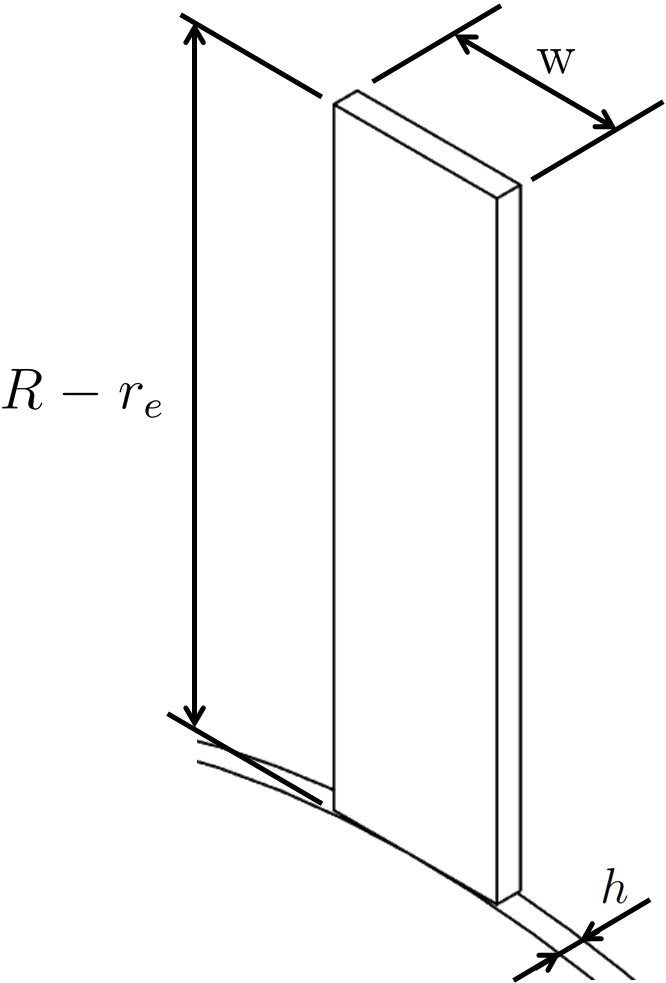
\includegraphics[scale=0.25]{parametric_blade}
	\caption{Parametric blade dimensions.}
	\label{fig:parametric_blade}
\end{figure}

Equation ~\ref{equation:volume_ratio} defines a relationship between the volume of the corresponding full ring prior to the machining of the blades, visualized in Figure ~\ref{fig:full_ring_prior_to_blade_machining}, and the total volume of the blades visualized in Figure ~\ref{fig:total_volume_of_blades}. 

\begin{figure}[h]
	\centering
	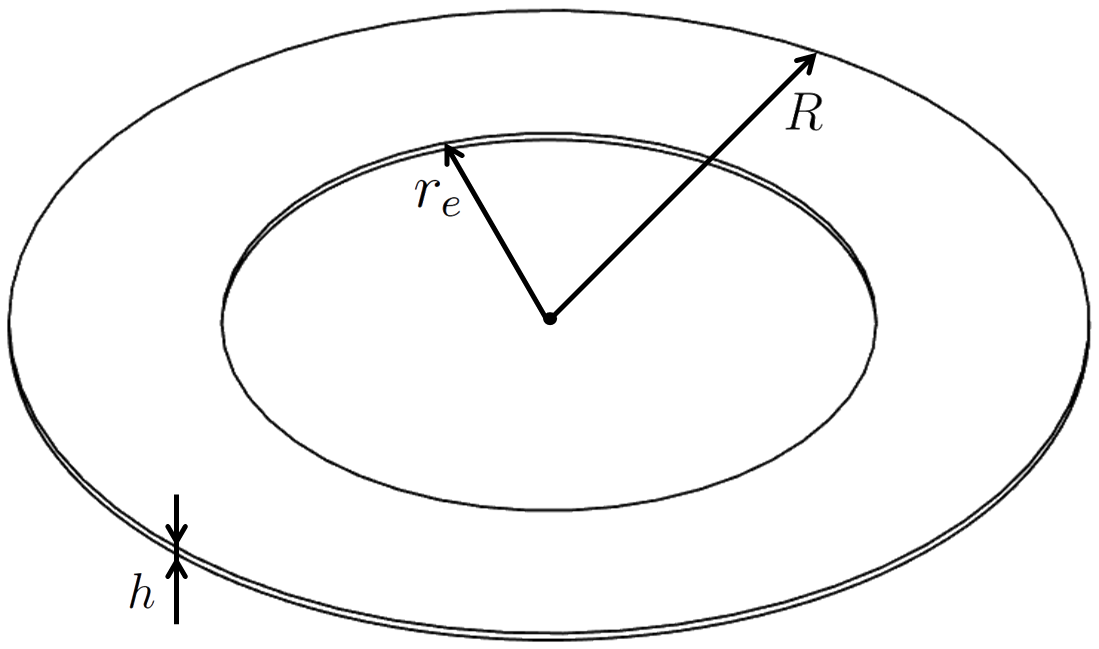
\includegraphics[scale=0.25]{full_ring_prior_to_blade_machining}
	\caption{The volume of the corresponding full ring prior to the machining of the blades.}
	\label{fig:full_ring_prior_to_blade_machining}
\end{figure}

\begin{figure}[h]
	\centering
	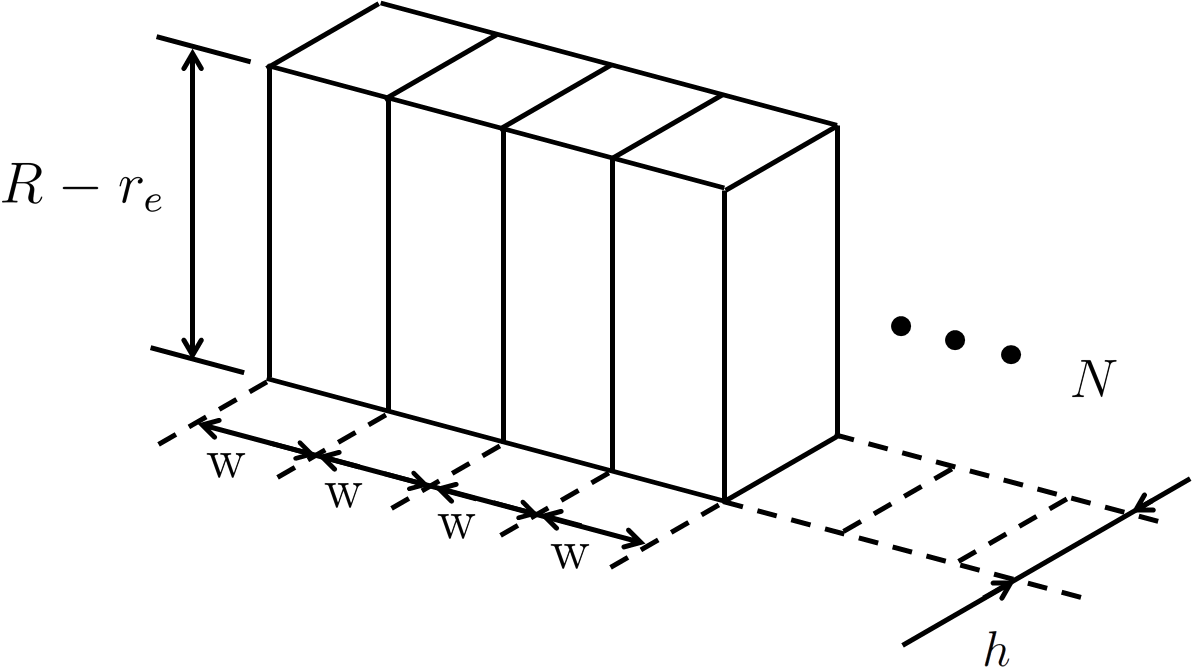
\includegraphics[scale=0.3]{total_volume_of_blades}
	\caption{The total volume of blades.}
	\label{fig:total_volume_of_blades}
\end{figure}

Equation ~\ref{equation:volume_ratio} is rewritten as

\begin{equation}
	\label{equation:v_ratio}
	V_{blades} = k V_{ring}.
\end{equation}

The volume of the corresponding full ring prior to the machining of the blades is

\begin{equation}
	\label{equation:v_ring}
	\begin{aligned}
		V_{ring} &= \pi R^2 h - \pi r_e^2 h \\
		&= \pi h (R^2-r_e^2).
	\end{aligned}
\end{equation}

The total volume of the blades is

\begin{equation}
	\label{equation:v_blades}
	V_{ring} = N \mathrm{w} h (R-r_e).
\end{equation}

The thickness of the plane stress elements in the finite element analysis is defined as

\begin{equation}
	\label{equation:t_ps_i}
	t = N \mathrm{w}.
\end{equation}

Substituting Eq. ~\ref{equation:t_ps_i} into Eq. ~\ref{equation:v_blades}, we have

\begin{equation}
	\label{equation:v_blades_t}
	V_{ring} = t h (R-r_e).
\end{equation}

Substituting Eqs. ~\ref{equation:v_blades_t} and ~\ref{equation:v_ring} into Eq. ~\ref{equation:v_ratio}, we have

\begin{equation}
	\begin{aligned}
		t h (R-r_e) &= k \pi h (R^2-r_e^2) \\
		t \cancel{h} \cancel{(R-r_e)} &= k \pi \cancel{h} \cancel{(R-r_e)} (R+r_e),
	\end{aligned}
\end{equation}

and

\begin{equation}
	\label{equation:t_ps}
	t = k \pi (R+r_e).
\end{equation}

The radial stress, hoop stress, and radial displacement results from CalculiX are shown in Figures, ~\ref{fig:graph_0},  ~\ref{fig:graph_1}, and  ~\ref{fig:graph_2}, respectively.

\begin{figure}[h]
	\centering
	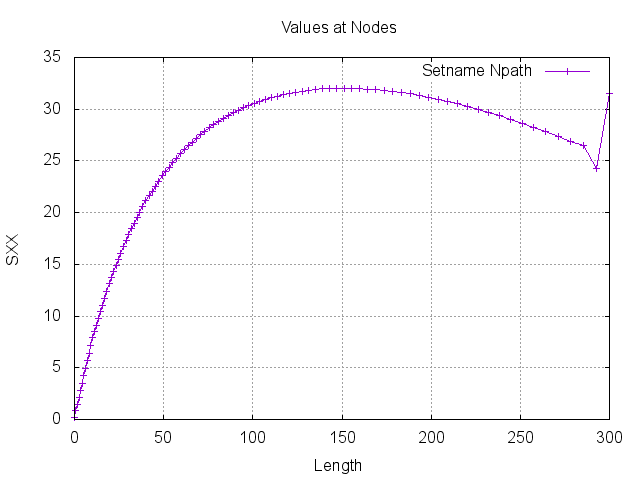
\includegraphics[scale=0.5]{graph_0}
	\caption{CalculiX radial stress plot.}
	\label{fig:graph_0}
\end{figure}

\begin{figure}[h]
	\centering
	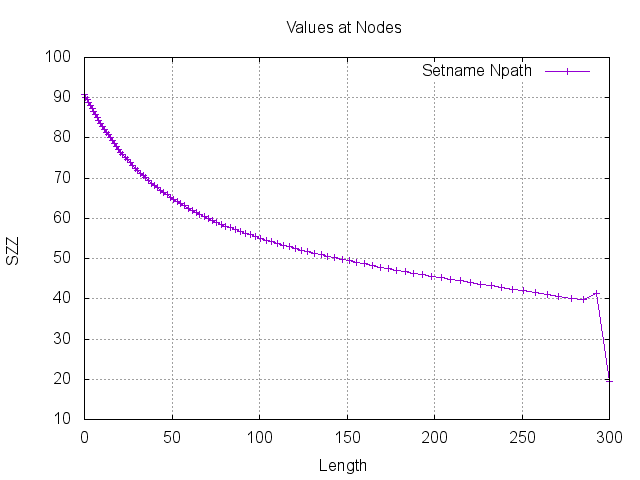
\includegraphics[scale=0.5]{graph_1}
	\caption{CalculiX hoop stress plot.}
	\label{fig:graph_1}
\end{figure}

\begin{figure}[h]
	\centering
	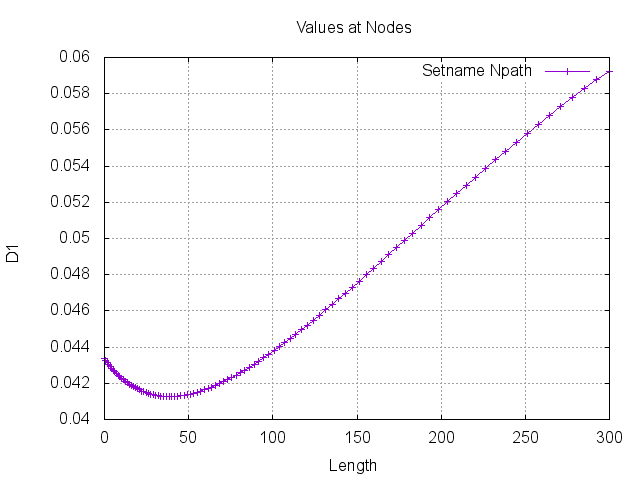
\includegraphics[scale=0.5]{graph_2}
	\caption{CalculiX radial displacement plot.}
	\label{fig:graph_2}
\end{figure}

\textbf{Summary:}\\

Maximum radial stress is 32 MPa.

Maximum hoop stress is 91 MPa.

Radial displacement at the inner radius is 0.043348 mm.

Radial displacement at the outer radius is 0.059241 mm.


\clearpage
\section{Comparison}
Dimensionless stresses and displacement are defined below (see Eqs. ~\ref{equation:dimensionless_sigma_r}, ~\ref{equation:dimensionless_sigma_t}, and ~\ref{equation:dimensionless_u_r}). 

\begin{equation}
\label{equation:dimensionless_sigma_r}
{ \overline{{\sigma }}_{r}=}{\frac {8} {(3+{\nu }){\rho }{{\omega }^{2}{r}^{2}_{e}}}}{\sigma }_{r}
\end{equation}

\begin{equation}
\label{equation:dimensionless_sigma_t}
{\overline{\sigma }_{t}=}{\frac {8} {(3+{\nu }){\rho }{{\omega }^{2}{r}^{2}_{e}}}}{\sigma }_{t} 
\end{equation}

\begin{equation}
\label{equation:dimensionless_u_r}
{\overline{u}_{r}=}{\frac {8E} {(3+{\nu })(1-{\nu }){\rho }{{\omega }^{2}{r}^{3}_{e}}}}{u}_{r}
\end{equation}\\

A MATLAB code is written to perform the following tasks:

\begin{itemize}
	\item Run a Python code that performs the following tasks:
	\begin{itemize}
		\item Run the pre-processing file that contains parametric model information. Create the geometry and mesh, and export the finite element pre-processing data in CalculiX format.
		\item Run the finite element input file in CalculiX.
		\item Run the post-processing file that generates result plots and saves them.
	\end{itemize}
	\item Load CalculiX results into MATLAB workspace,
	\item Define the problem geometry with given parametric values for analytical solution.
	\item Calculate the analytical results for radial stresses, hoop stresses, and radial displacements and plot them.
	\item Derive the dimensionless stresses, and displacements from the analytical and CalculiX results, and compare them in a single plot, from $r_i$ to $r_e$.
\end{itemize}

The comparison between the analytical solution and the finite element results obtained from CalculiX is presented in Figure ~\ref{fig:blisk_analytical_vs_fe}. It can be observed that the finite element results from CalculiX are the same as the analytical solution except in the very close proximity to the plane stress elements.

\clearpage
\begin{landscape}
	\begin{figure}[h]
		\centering
		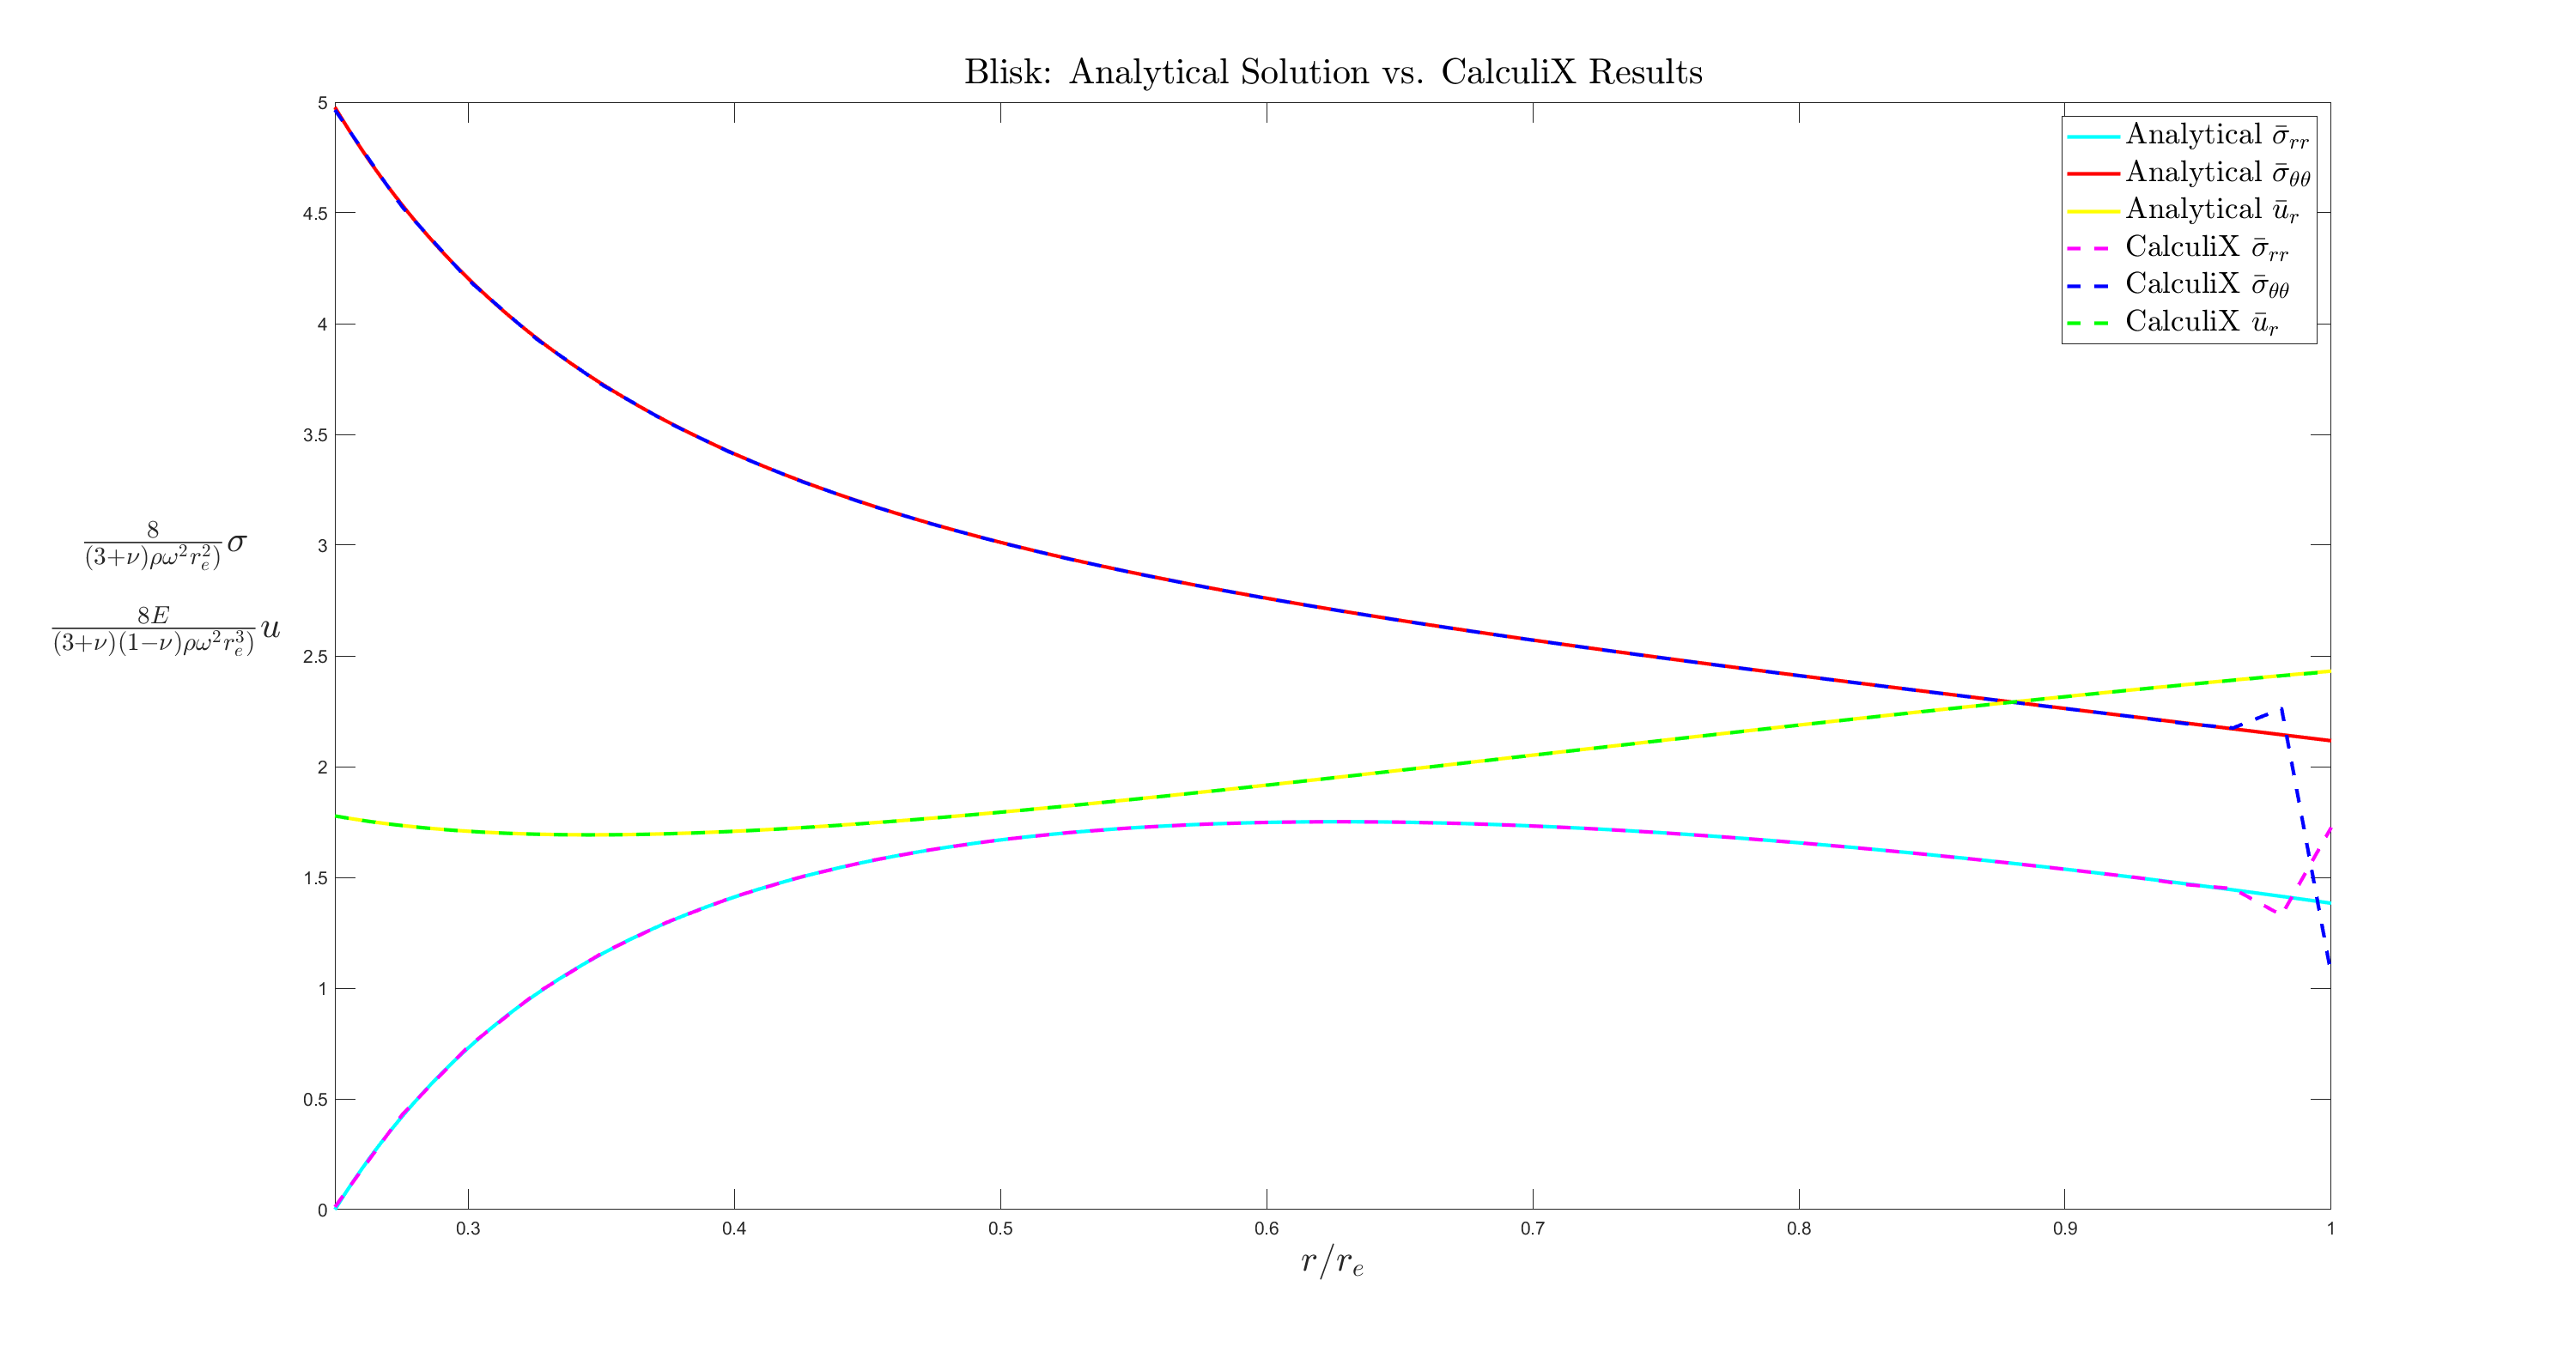
\includegraphics[scale=0.5]{blisk_analytical_vs_fe}
		\caption{Two-dimensional rotating blisk: Analytical solution vs. CalculiX results.}
		\label{fig:blisk_analytical_vs_fe}
	\end{figure}
\end{landscape}

\clearpage
% Bibliographic references
\begin{thebibliography}{9}	
	\bibitem{rotors_book} 
	Rotors: Stress Analysis and Design, 2013. Page 39, Example 4. 
	
	\bibitem{CalculiX_website} 
	CalculiX, A Free Software Three-Dimensional Structural Finite Element Program. \url{http://www.calculix.de/}
\end{thebibliography}


\end{document}